\section{O-løb}
Følgende afsnit vil omhandle hvad et o-løb er, termer fra sporten og forklare hvordan et typisk o-løb fungere. Denne information er fundet på Dansk Orienterings-Forbunds hjemmeside \citep{DOF}, samt interviews med Jens Børsting, der blev introduceret i indledningen, og Claus Bobach, som er klubtræner hos Aalborg Orienteringsklub.

O-løb er en sport hvor det, som så mange andre sportsgrene, gælder om at være hurtigst. O-løb er anderledes, da det er op til løberen selv at finde vej, ved hjælp af et kort, og måske et kompas. Inden løbet starter, bliver alle løbere udstyret med et kort, med detaljeret visning af stier, bakker og andre udfordringer i terrænet. På dette kort vises de forskellige poster løberen skal finde inden vedkommende har gennemført løbet. Hvis kortet viser en bestemt rækkefølge posterne skal besøges i, så er det påkrævet at gøre det i den rækkefølge. 

Kortlæsning er en af de vigtigste aspekter ved o-løb. Det gør løberen i stand til at finde rundt, optimere sin rute og vælge den bedste vej rundt om forhindringer. ”Vi kan med god ret sige, at det er her sjælen i sporten ligger gemt”, skriver Dansk Orienterings-Forbund.   

Ved hver post, står en orange/hvid skærm (figur 2.1). På skærmen er oplyst et nummer, så det er muligt at tjekke om det er den rigtige post der er fundet. Desuden er der ved mange løb opstillet elektronisk poster, (figur 2.2) som gør det muligt at se hvornår løberen har været ved posterne.

\begin{figure}
	\centering
	\begin{minipage}{.5\textwidth}
		\centering
		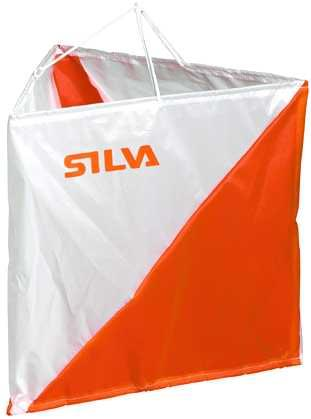
\includegraphics[width=.5\linewidth]{billeder/o-skaerm}
		\caption{Almindelig skærmpost}
		\label{fig:test1}
	\end{minipage}%
	\begin{minipage}{.5\textwidth}
		\centering
		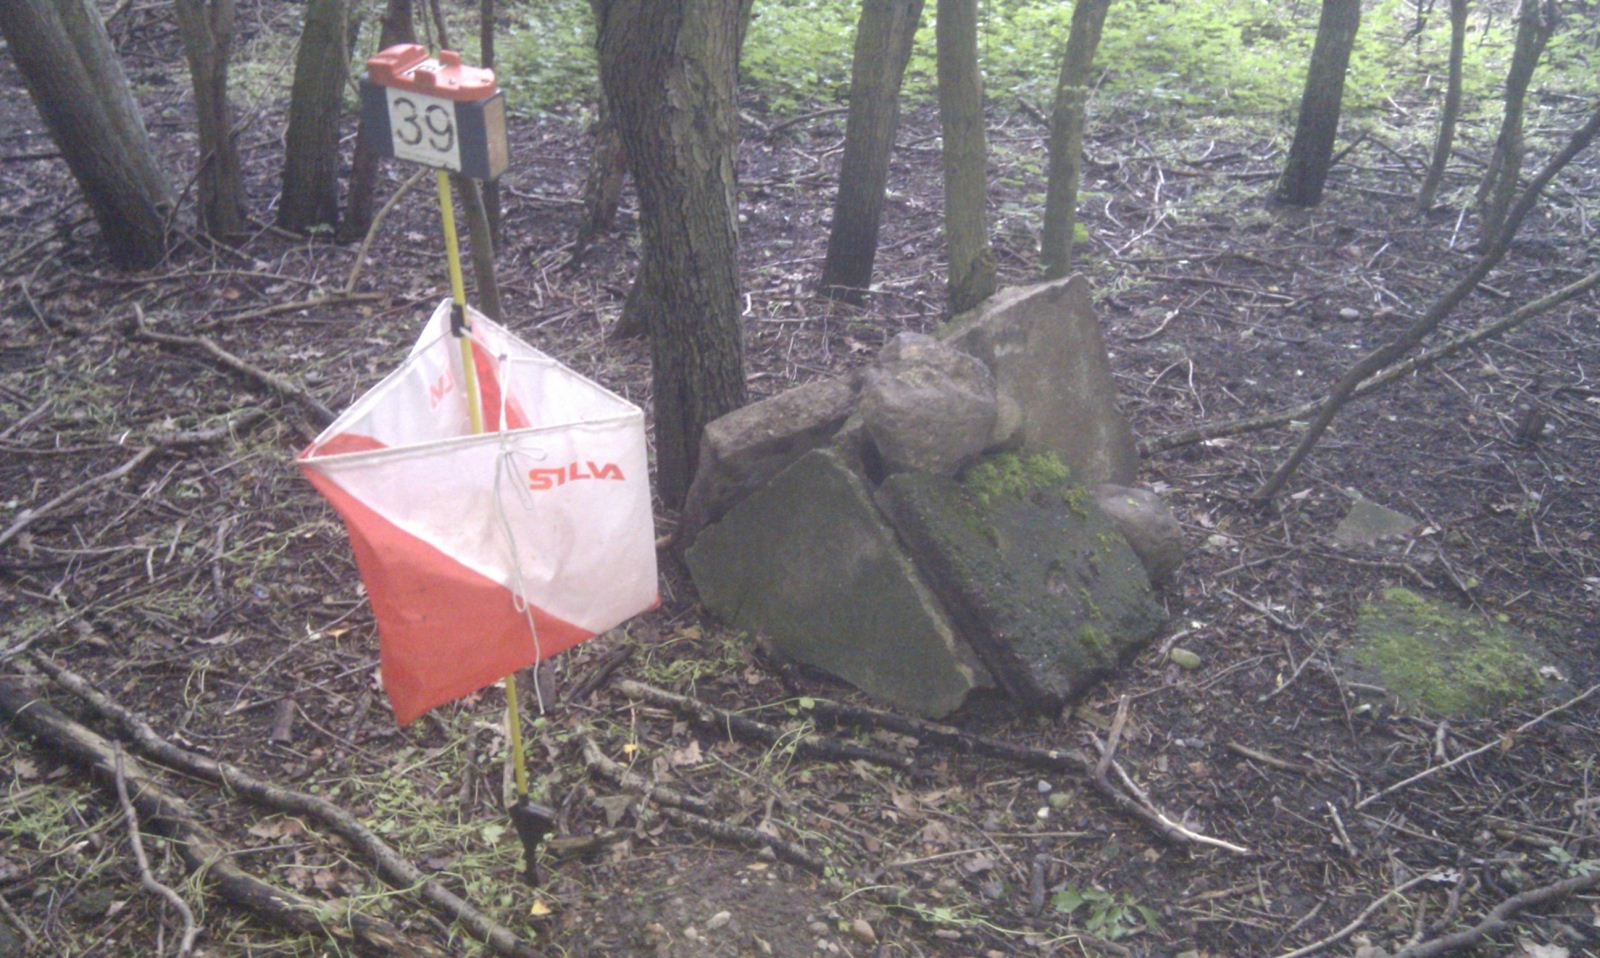
\includegraphics[width=1.0\linewidth]{billeder/banelaeggerkreativitet}
		\caption{Elektronisk post}
		\label{fig:test2}
	\end{minipage}
\end{figure}
Der findes en række forskellige discipliner inden for o-løb. Først er der Sprint, Mellem, Lang og Ultralang, der er enkeltmandsløb, hvor den eneste forskel er distancen der løbes. Sprint er den korteste, og blive ofte afviklet i byer for at gøre det så simpelt og hurtigt som muligt, og Ultralang er den længste, hvor vindertiden typisk er højere end ved maratonløb. Udover standard løbene, findes også Nat, Stafet og Hold, der adskiller sig ved, henholdsvis at foregå om natten, eller have flere løbere. 
